\section{Měření polohy - principy odporové, indukčnostní, kapacitní}
\subsection{Odporové snímače polohy}

\subsubsection{Snímače se skokovou změnou odporu}
Mechanicky ovládané kontakty:
\begin{itemize}
    \item Mechanické mikrospínače - ovládání světla
    \item Parametry: Rozsahy síly potřebné pro spínání, velikost proudu/napětí které mohou spínat(větší problém s DC proudy), životnost z pohledu počtu spínání(rychlost mechanické únavy, klasicky \(10^6\) sepnutí)
\end{itemize}
Magneticky ovládané kontakty:
\begin{itemize}
    \item Jazýčková relé - kontakty z magneticky měkkého materiálu ovládané polem permamentního magnetu
    \item Princip - k relé přibližujeme magnet, přiblížením vzniká přitažlivá síla mezi kontakty relé
    \item Parametry - spínané proudy(jednotky mA), max počet přepnutí
    \item Kontakty se mohou slepit kvůli přiliš silné magnetizaci
    \item Měření rychlosti na kole, otevření zavření dveří, atd...
\end{itemize}
\begin{figure}[h!]
    \centering
    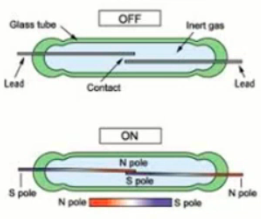
\includegraphics[scale = 0.5]{img/JazRele.png}
\end{figure}
\subsubsection{Snímače s plynulou změnou odporu}
Odporové potenciometry s pohyblivým kontaktem mechanicky spojeným s měřenou veličinou.\\
Na nevodivé podložce je nanesena vodivá vrstva, přes kterou přejíždí pohyblivý kontakt a měříme odpor mezi jezdcem a jedním z okraju vodivé dráhy.\\
Dělení podle typu jezdce:
\begin{itemize}
    \item Rotační jezdec - měření úhlového posunutí
    \item Přímočarý jezdec - měření polohy nebo lineárního posunutí
    \item Spirálový jezdec - helipot typicky s 10 závity, rozsah větší jak 360°
\end{itemize}
Lankem ovládané potenciometry, mají rozsah až 40m, rychlost 2m/s.
\begin{figure}[h!]
    \centering
    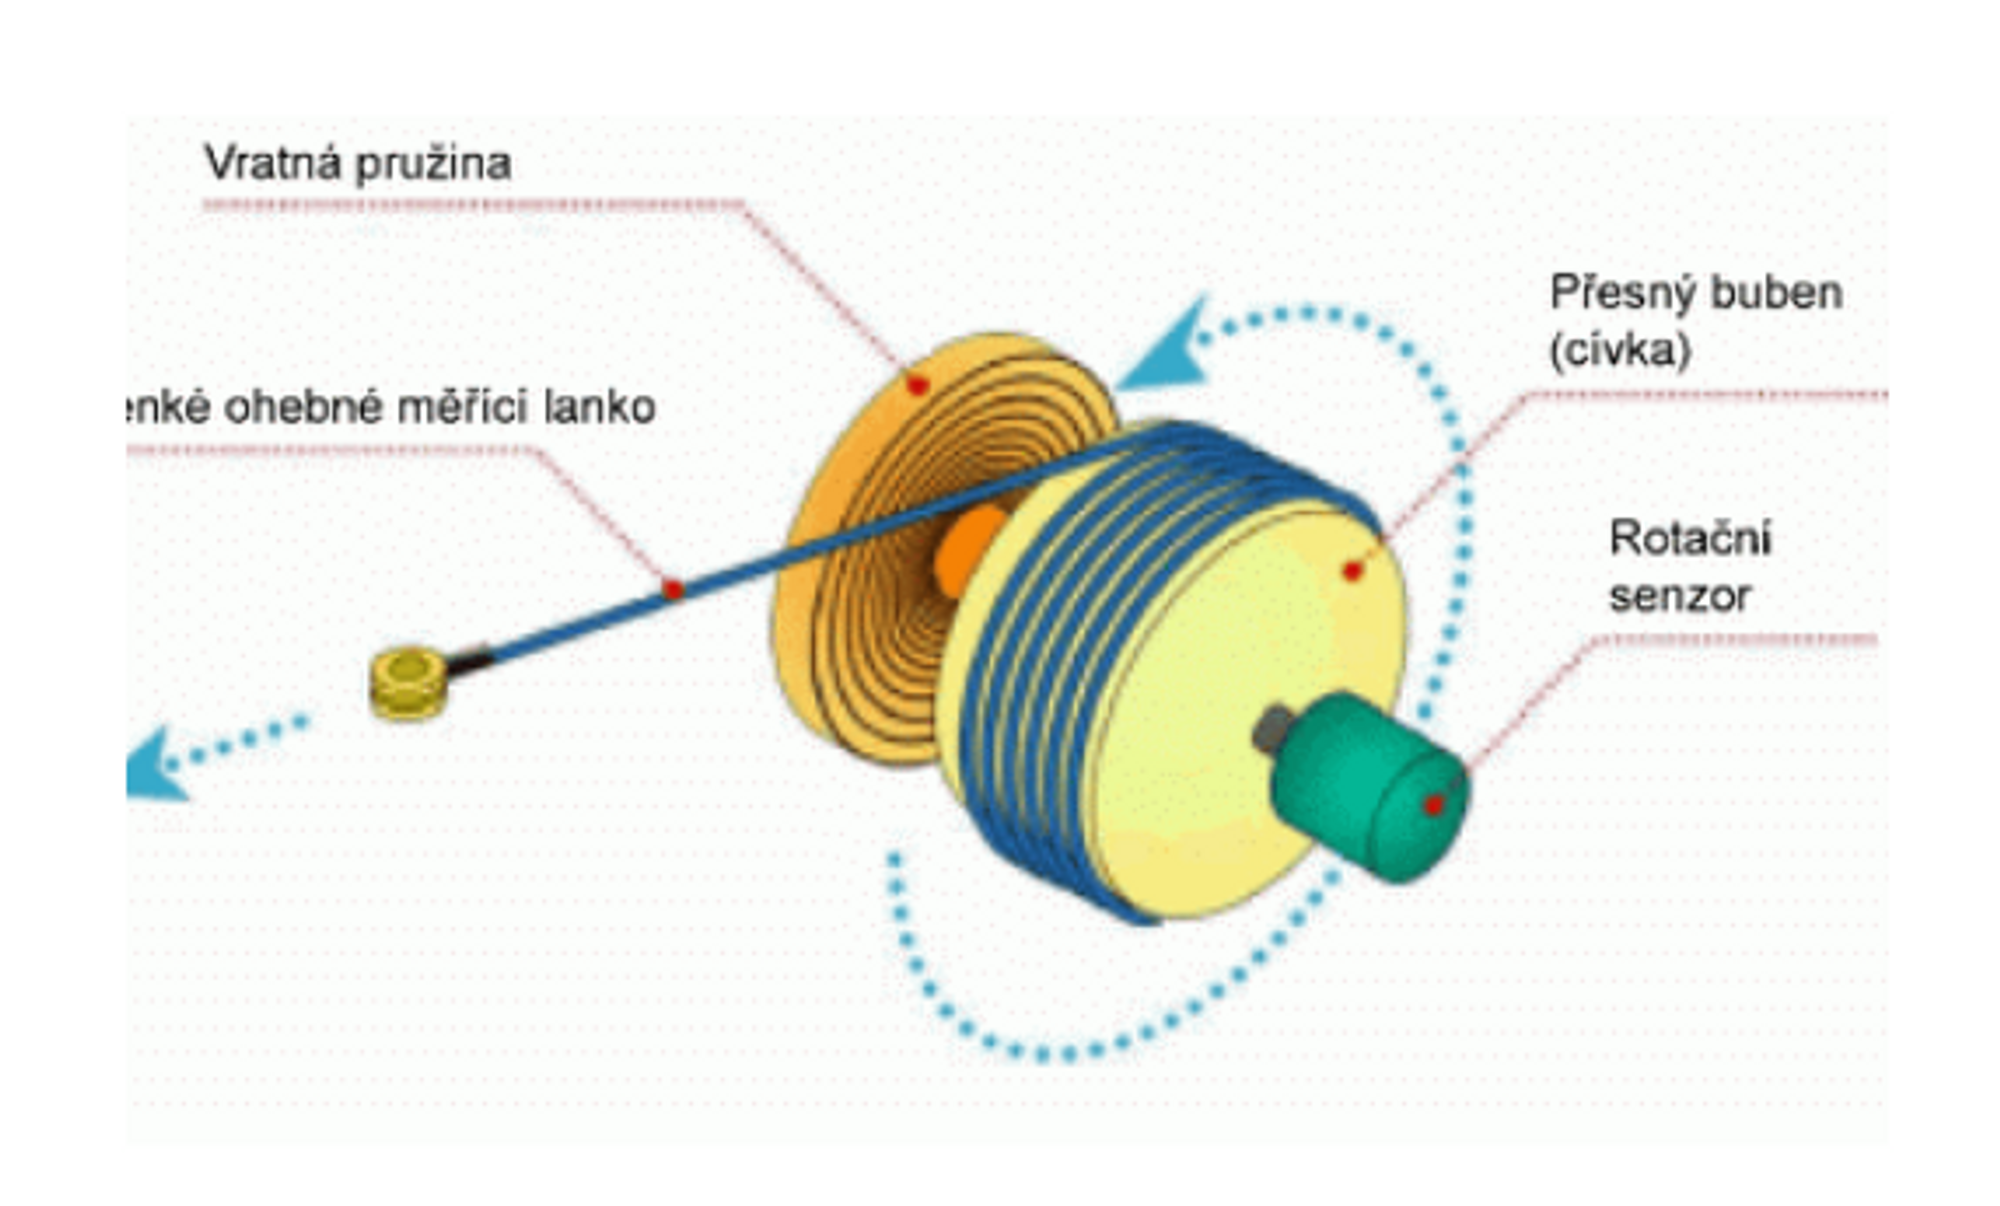
\includegraphics[scale = 0.1]{img/Lanko.png}
\end{figure}

\subsubsection{Zapojení odporových snímačů}
\begin{figure}[h!]
    \centering
    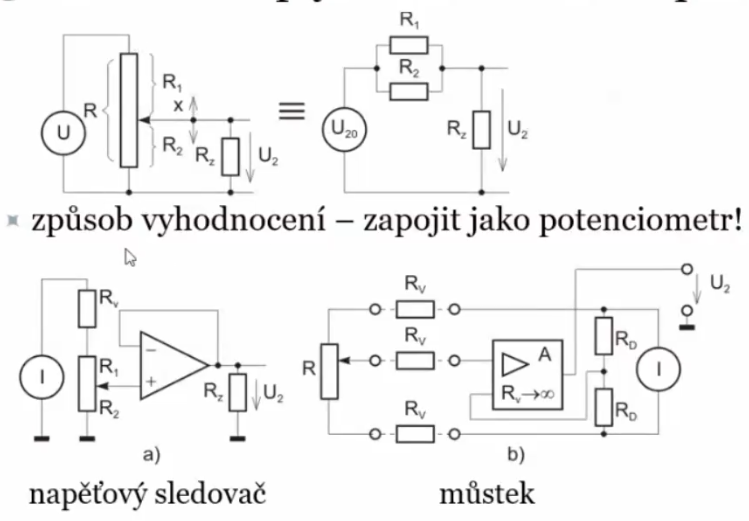
\includegraphics[scale = 0.4]{img/ZapojOdp.png}
\end{figure}
V prvním zapojení je \textit{R} samotný snímač, který se připojí na ke zdroji U, tím se stanoví rozsah a potom posouváním, které je zobrazeno proměnnou x měníme odpor. Měříme výstupní napětí \(U_2\)\\
Požadavek, aby výstupní dělič byl nezatížený, chceme aby vstupní odpor voltmetru byl poměrně veliký.\\
Je nutno zajistit aby odběr proudu z děliče byl co nejmenší, jinak se bude chovat nelineárně. To se dá řešit buď vysokým vstupním odporem voltmetru anebo napěťovým sledovačem. Pokud má voltmetr odpor větší jak 1:100 vůči měřicí kartě už nám na tomto nezáleží.\\
V zapojení napěťového sledovače je mezi zátěžový odpor a snímač zaveden napěťový zesilovač s jednotkovým zesílením. Ideální zesilovač má nekonečný vstupní a nulový výstupní odpor, což vede k tomu, že na zátěžovém odporu nezáleží.\\
Můstek, pokud máme dlouhé vodiče od snímače kde se začne projevovat odpor vodičů, výhodou je že potlačuje odpor vodičů \(R_v\).
\subsubsection{Výhody}
\begin{itemize}
    \item jednoduché zpracování signálu
    \item jednoduchá výroba, levné
    \item reprodukovatelnost, linearita
    \item odolnost proti vibracím - ne tak uplně, jen běžné průmyslové vibrace tlumí
\end{itemize}
\subsubsection{Nevýhody}
\begin{itemize}
    \item kontaktní princip
    \item šum
    \item životnost
    \item dynamické vlastnosti - kvůli mechanickým vlastnostem, měřitelná pouze pomalá změna
    \item omezený ztrátový výkon(vnitřní odpor děliče musí být menší než vstupní odpor aby nedocházelo k přehřívání)
\end{itemize}

\subsection{Indukčnostní snímače polohy}
Pasivní snímače, měřená veličina je převáděna na změnu indukčnosti(jedna nebo dvě cívky) nebo vzájemné indukčnosti(dvě nebo tři cívky).\\
Dělení indukčnostních snímačů:
\begin{itemize}
    \item Dle magnetického obvodu:
          \begin{itemize}
              \item S otevřeným magnetickým obvodem - magnetický tok prochází z velké části vzduchem
              \item S uzavřeným magnetickým obvodem - magnetický tok prochází z velké části přes magneticky vodivý materiál
          \end{itemize}
    \item Dle uspořádání cívek:
          \begin{itemize}
              \item Jednoduchá(parametrický) snímač - změna indukčnosti 1 cívky, závislost nelineární
              \item Diferenční snímač - vyhodnocujeme rozdíl dvou cívek
              \item Transformátorový snímač - 1 cívka napájecí, měříme změnu vzájemné indukčnosti napájecí s dvuma cívkama sekundárníma
          \end{itemize}
    \item Dle principu:
          \begin{itemize}
              \item Změna indukčnosti
              \item Změna vzájemné indukčnosti - LVDT, oscilátorové
          \end{itemize}
\end{itemize}

\subsubsection{Impedance cívky snímače}
\begin{center}
    \(Z(j\omega) = R + j\omega\frac{N^2}{Z_m} = R +j\omega\frac{N^2}{R_m+jX_m} = (R+ \frac{N^2\omega X_m}{\left\lvert Z_m(j\omega)\right\rvert^2 }) + j(\frac{N^2\omega R_m}{\left\lvert Z_m(j\omega) \right\rvert^2})\)
\end{center}
Kde:
\begin{itemize}
    \item R je ohmický odpor vinutí
    \item \(R_m\) a \(X_m\) jsou činná a jalová složka magnetické reluktance \(Z_m\). \(X_m = \frac{P_0}{\omega \Phi^2}\) odpovídá ztrátám vířivými proudy a hysterzí. U snímačů s vnesenou impedancí, snímačů s vířivými proudy, snímačů s potlačeným polem. \(R_m = \sum \frac{l_i}{\mu_i S_i}\) odpovídá geometrii uzavřeného magnetického obvodu. snímače s proměnnou délkou střední siločáry \(l_i\), snímače s proměnnou plochou \(S_i\) vzduchové mezery, snímače s proměnnou permeabilitou \(\mu_i\).
\end{itemize}
\begin{center}
    \(L \approx \frac{N^2}{R_m}\)
\end{center}
\subsubsection{Indukční snímač s uzavřeným magnetickým obvodem}
\subsubsection*{Indukčnostní snímač s proměnnou vzduchovou mezerou}
Jednoduchý parametrický snímač s proměnnou délkou střední siločáry ve vzduchové mezeře.\\
U \(R_m\) můžeme vypustit "kovovou" část, protože děláme permeabilitou železa, která je cca 300k a tím pádem je ten zlomek zanedbatelný oproti vzduchové části.\\
Nezávislý na parazitních vlivech.\\
\newpage
\begin{figure}[h!]
    \centering
    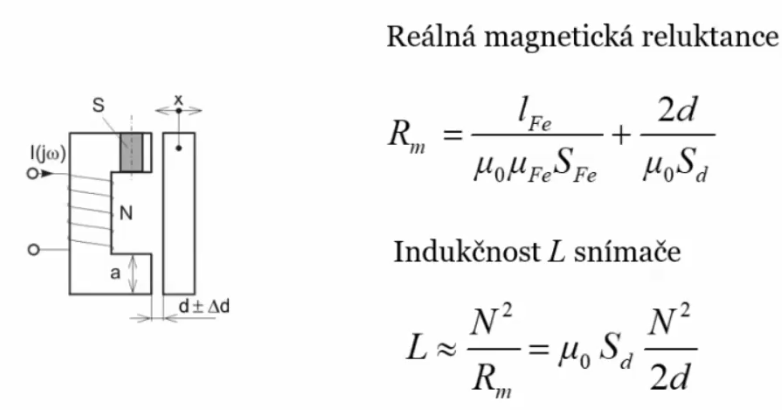
\includegraphics[scale = 0.3]{img/IndukcSPromMez.png}
\end{figure}

Diferenční snímač, přidáme stejný systém na druhou stranu (symetricky). Poté budem porovnávat rozdíl indukčností obou částí.\\
Při pohybu větší indukčnost bude na straně bude vzduchová mezera (d) menší.\\
Velmi jednoduchý,stabilní, robustní a má velkou citlivost(až extrémní).\\
Změna indučknosti napravo oproti te nalevo - můstkové zapojení.\\
\begin{figure}[h!]
    \centering
    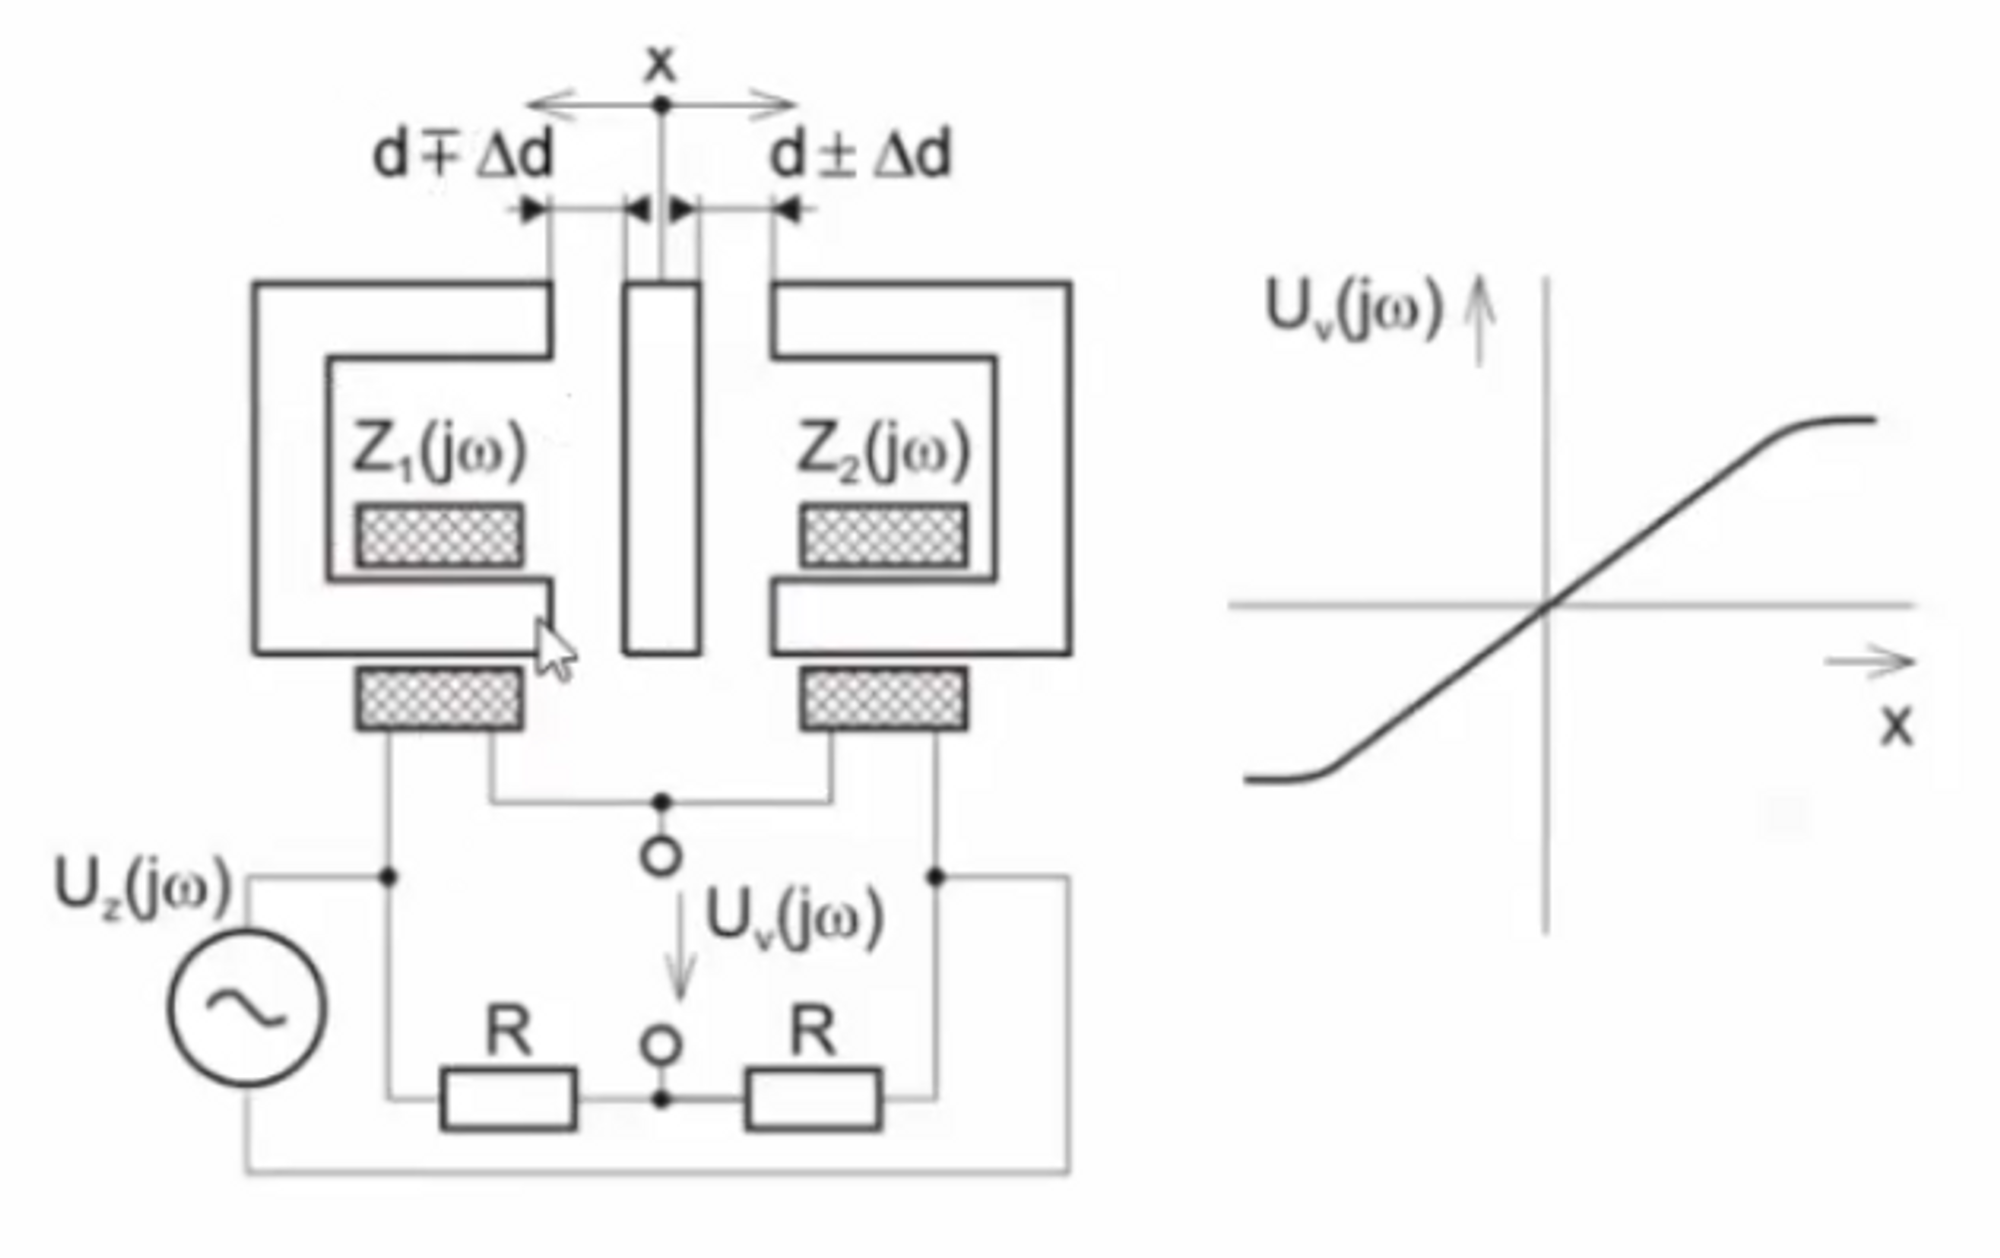
\includegraphics[scale = 0.1]{img/IndukDif.png}
\end{figure}
\subsection{Kapacitní snímače polohy}
Základní vztah:
\begin{center}
    \(C = \varepsilon \frac{S}{d} = \varepsilon_r \cdot \varepsilon_0 \frac{S}{d}\)
\end{center}
kde \(\varepsilon\) je permitivita, \(S\) je plocha elektrod a \(d\) je vzdálenost elektrod.\\
\begin{figure}[h!]
    \centering
    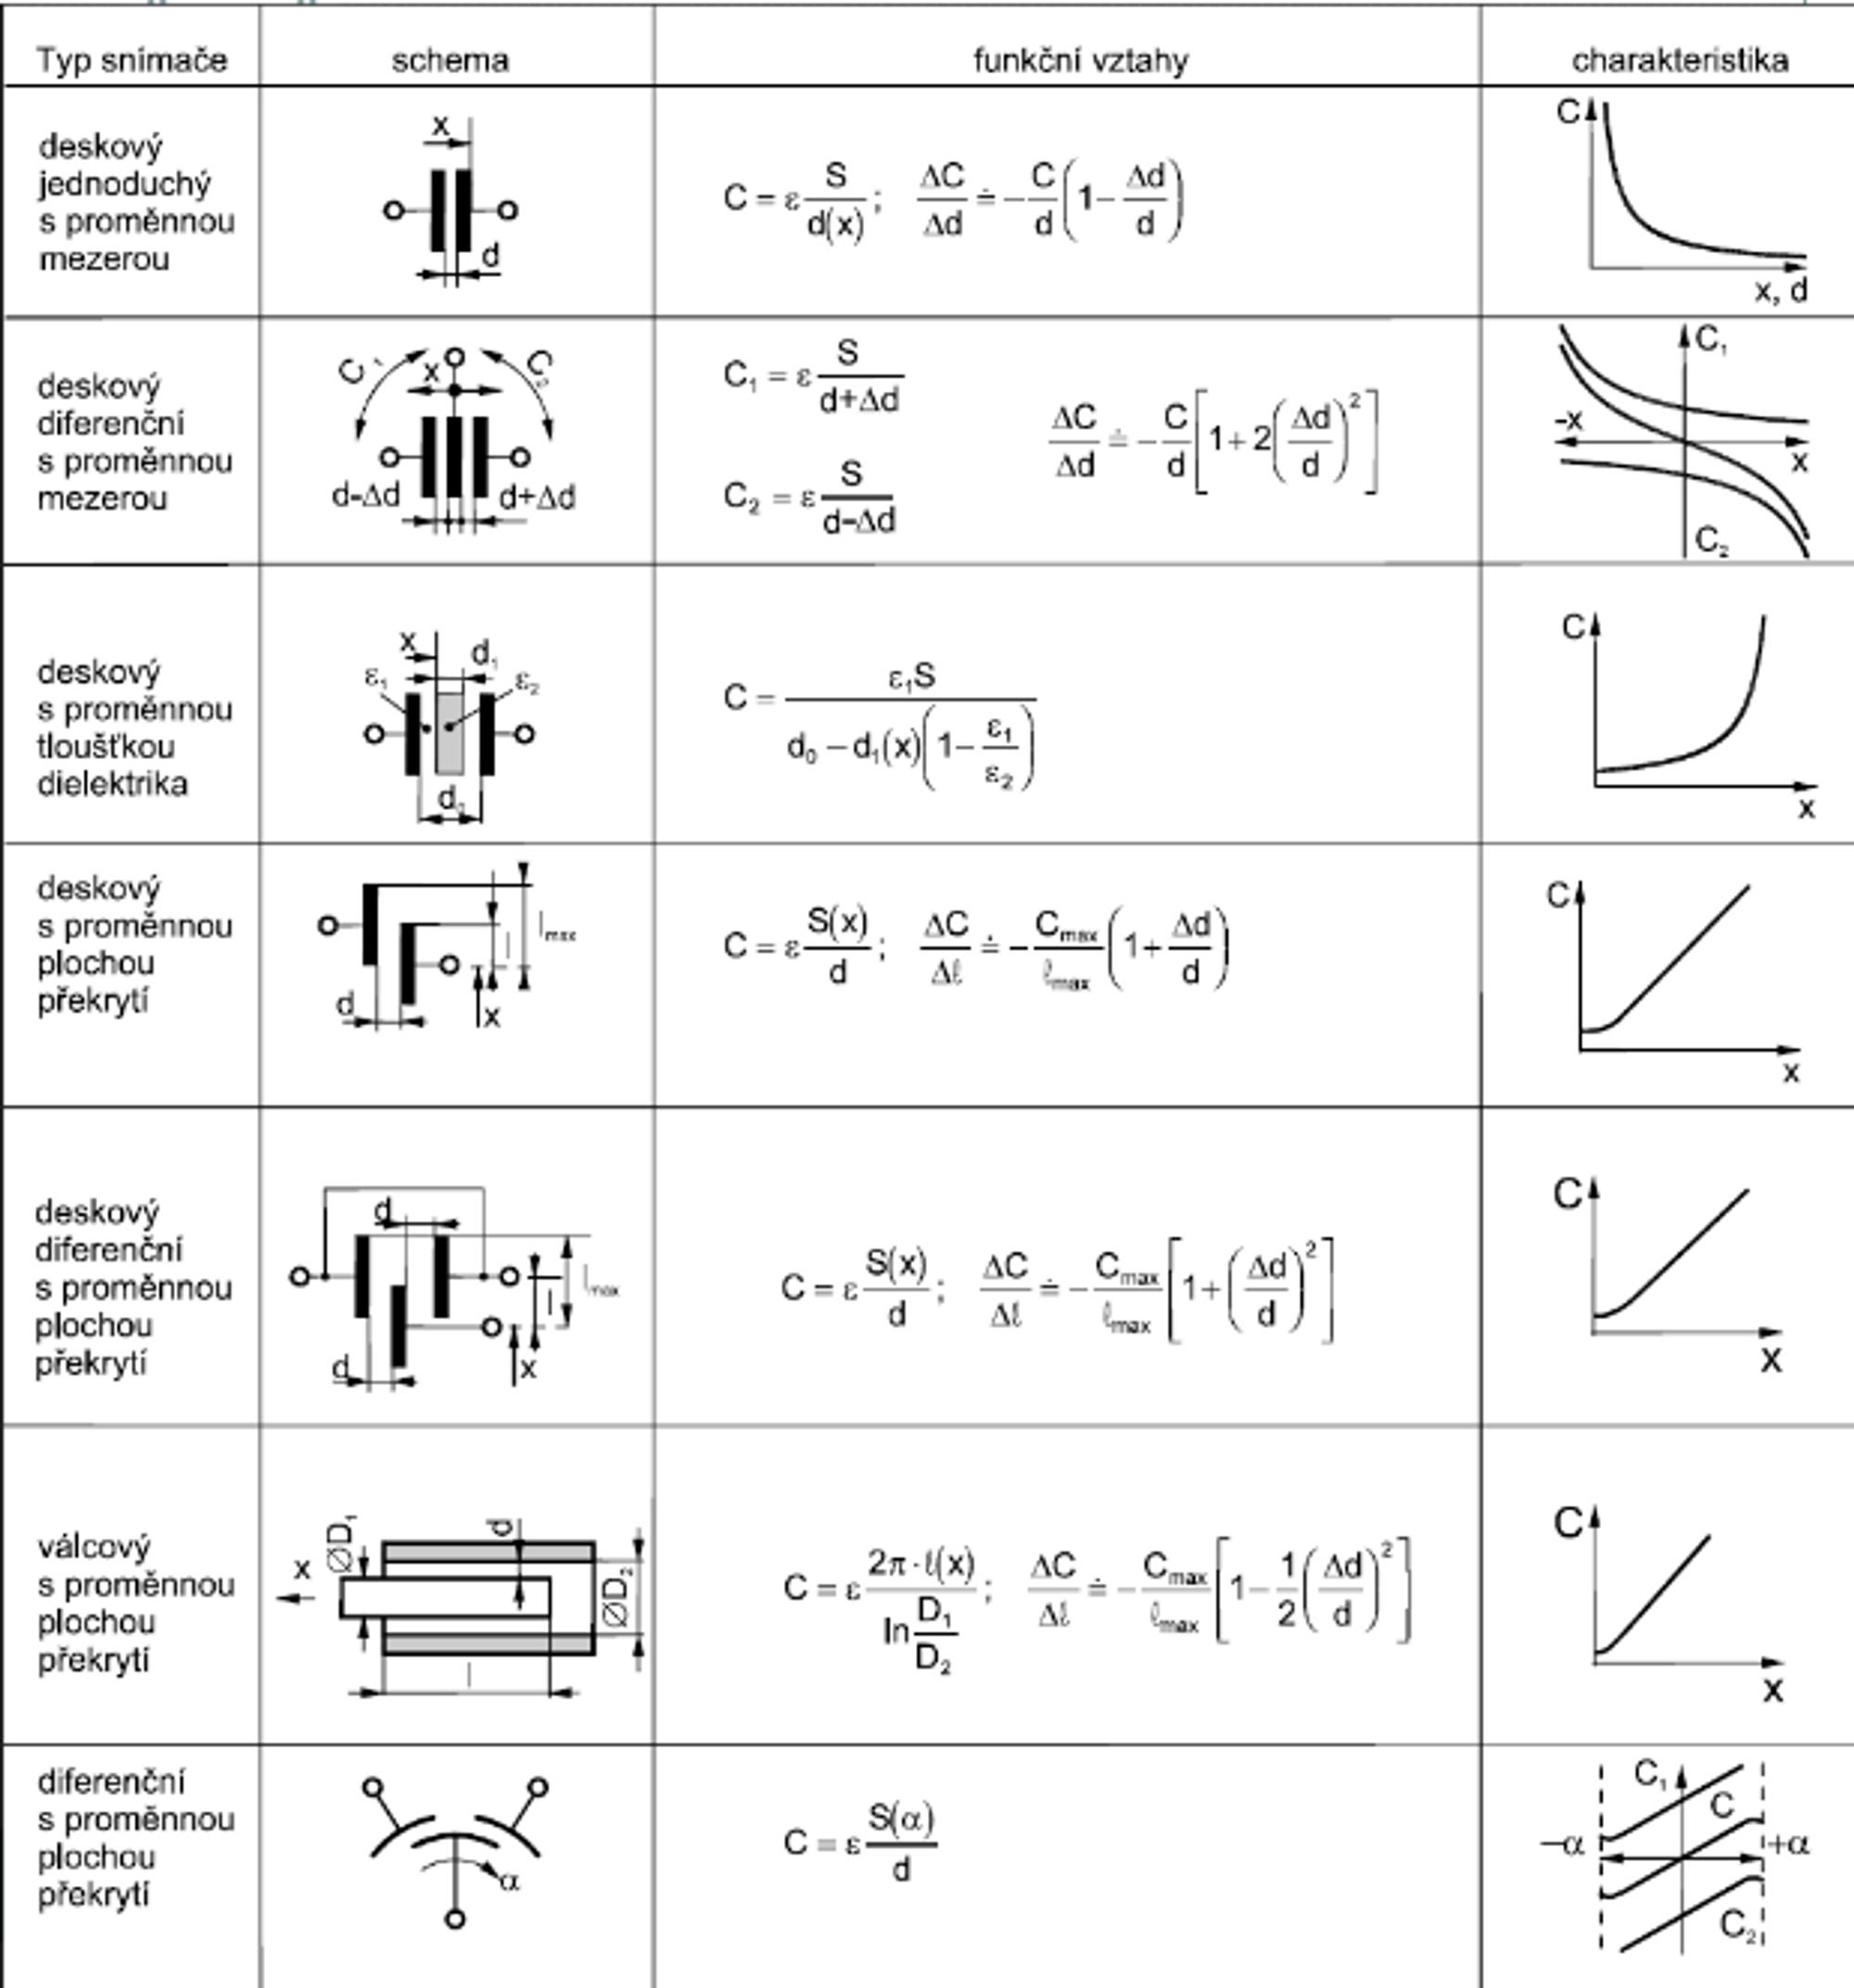
\includegraphics[scale = 0.1]{img/KapTypy.png}
\end{figure}
\subsubsection{Kapacitní senzor s proměnnou plochou překrytí}
\(C = \varepsilon \frac{S}{d}\).\\
Elektrody 1,2 pevné a elektroda 3 se pohybuje, vyhodnocujeme rozdíl.
\begin{center}
    Příklad vyhodnocení: \(\frac{C_{23}-C_{13}}{C_{23}+C_{13}}\)
\end{center}
Vzájemný poměr nezáleží ani na vzdálenosti, ani na permitivitě, tím potlačujeme téměř všechny parazitní vlivy, které nám zásadně ovlivňují měření.\\
\begin{figure}[h!]
    \centering
    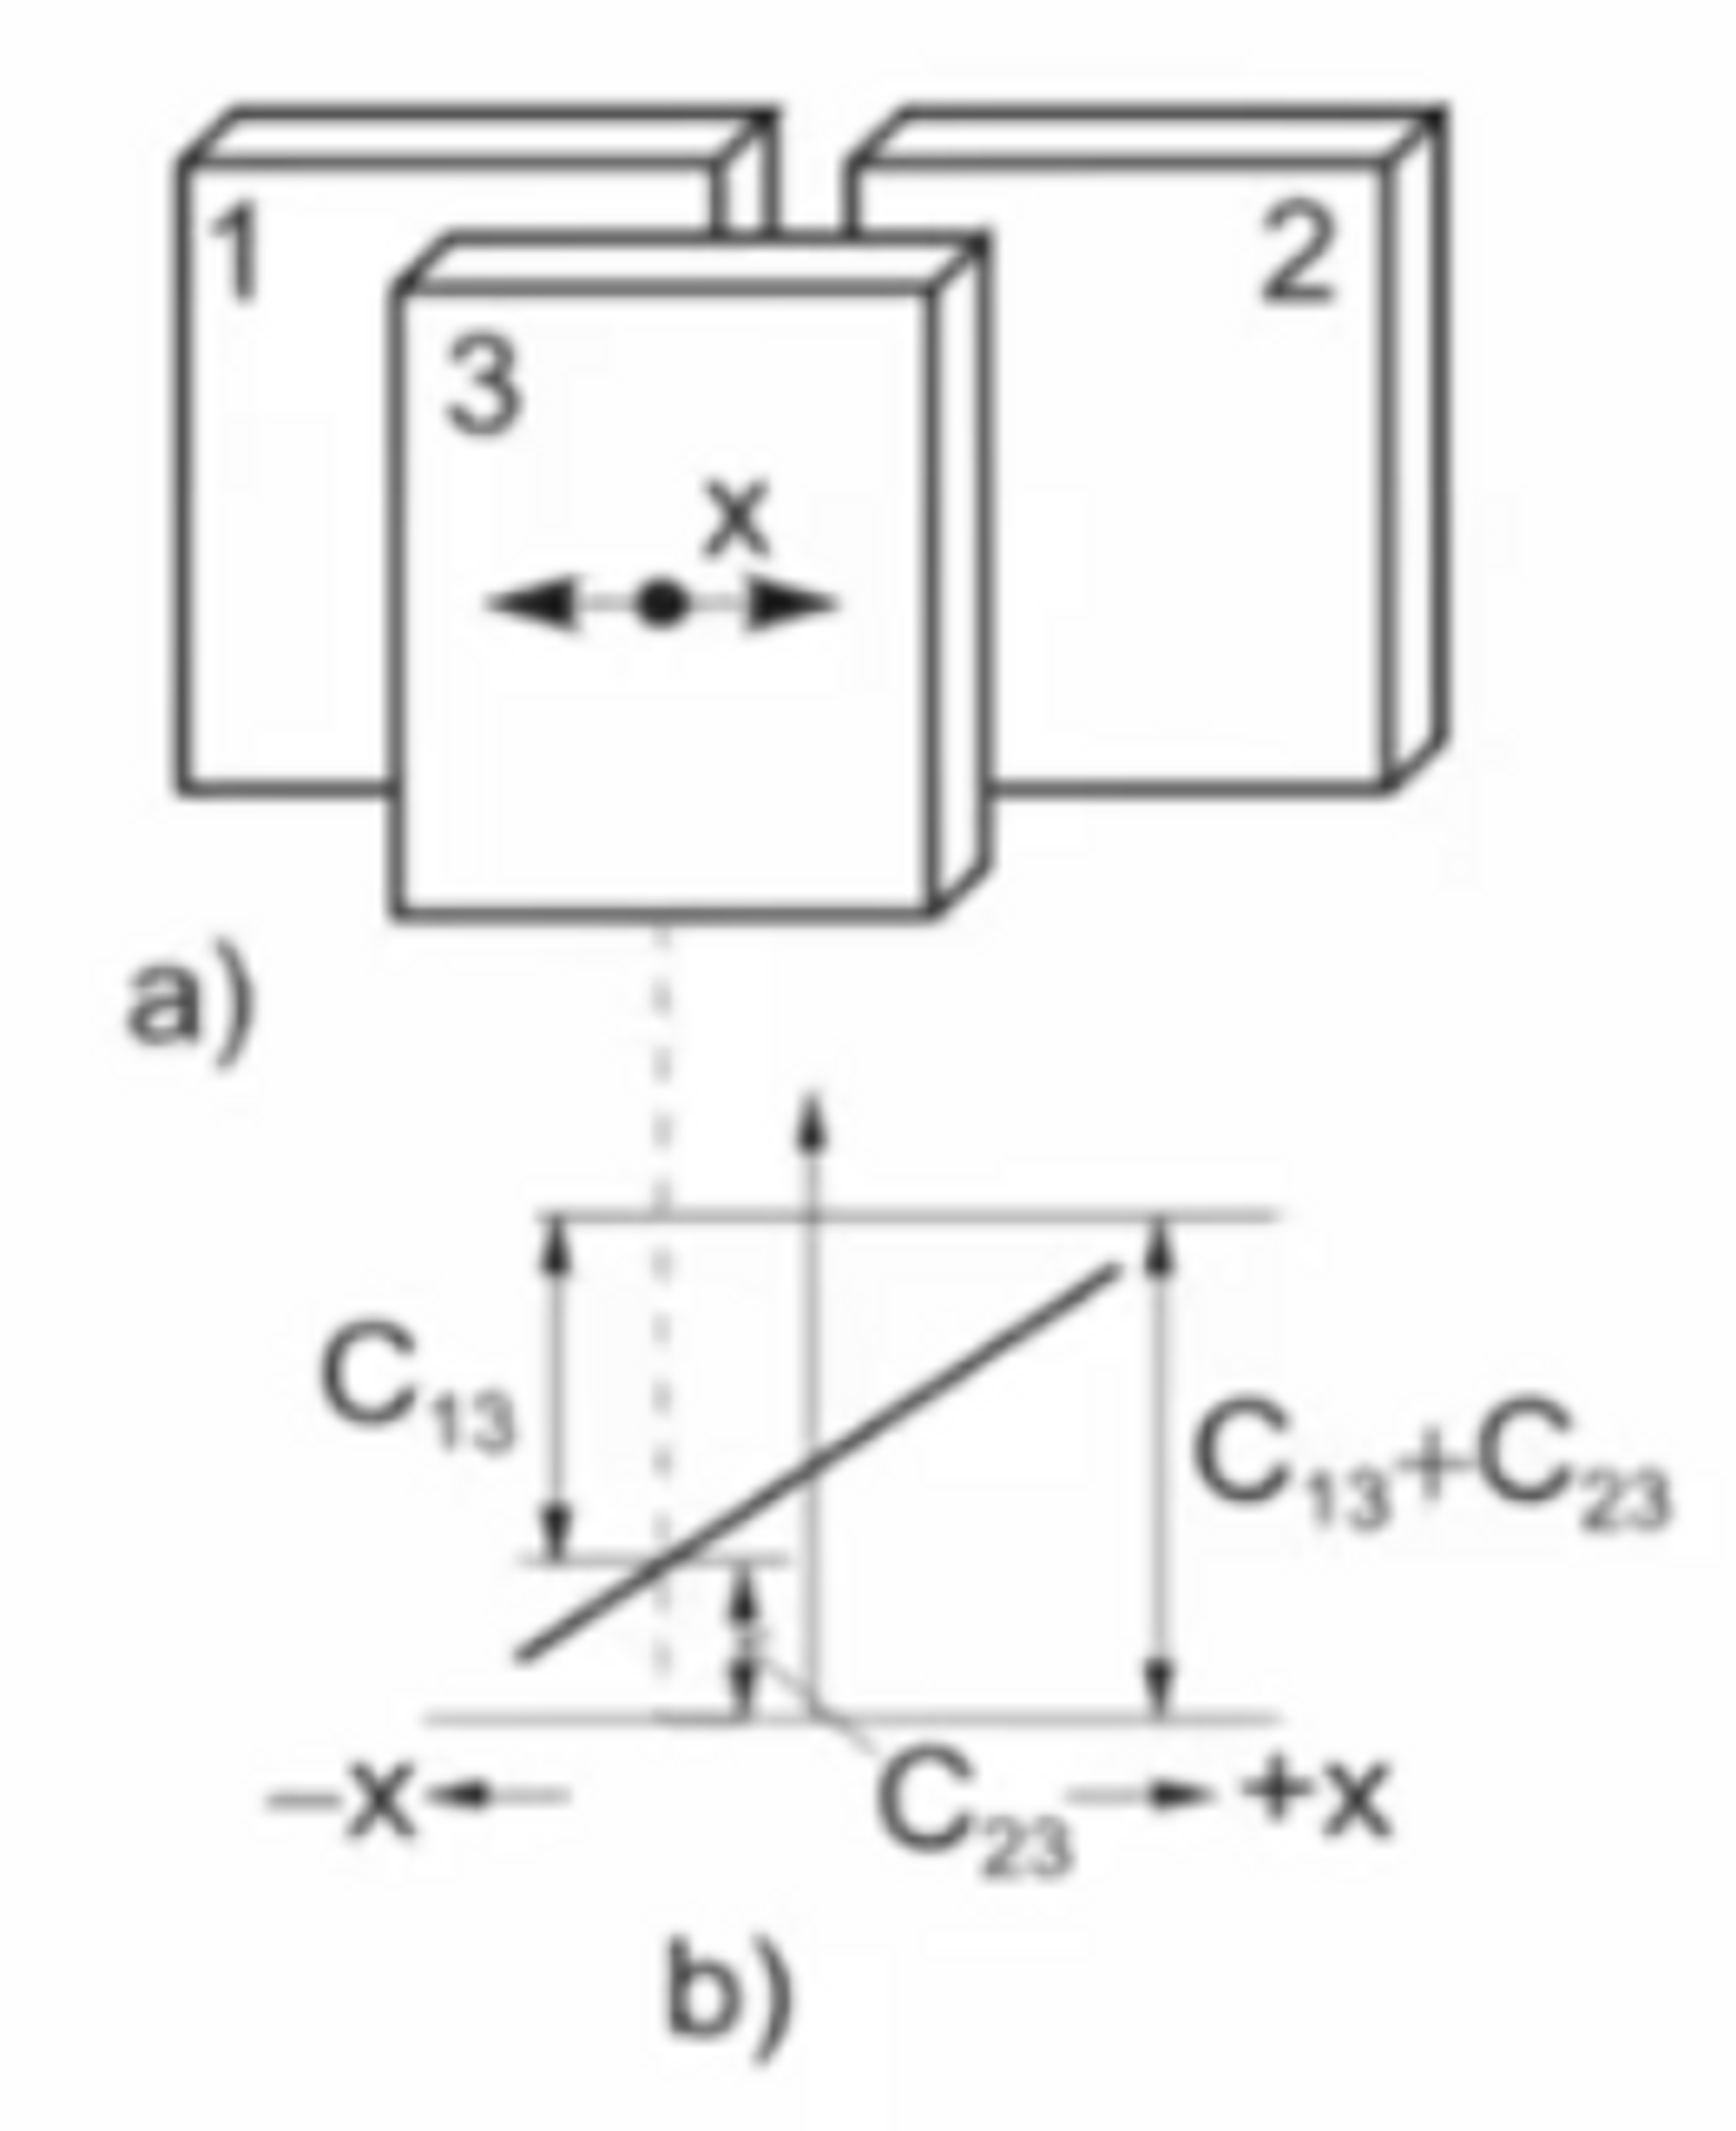
\includegraphics[scale = 0.07]{img/KapPromPloch.png}
\end{figure}

Vyhodnocení musí být provedeno v bezprostředné blízkosti elektrod. Kvůli malým kapacitám, se kterými se pracuje, by se projevoval vliv kabelů a naopak vliv elektrod by byl zanedbatelný.\\
Například v posuvném měřítku. V pevné části hodně elektrod a v posuvné jedna, kde díky změně kapacity měříme vzdálenost.\\

\subsubsection{Bezkontaktní snímače}
\begin{figure} [h!]
    \centering
    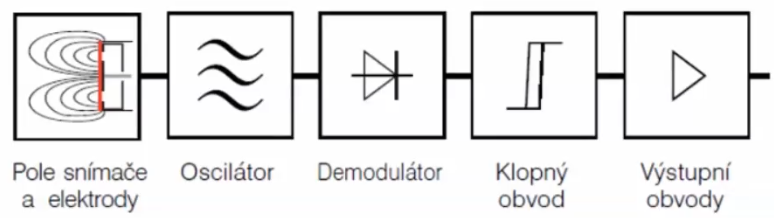
\includegraphics[scale = 0.3]{img/BezkonKap.png}
\end{figure}
Aktivní část tvoří 2 elektrody rovinného deskového kondenzátoru. Které jsou připojeny na oscilátor. Při přiblížení předmětu se naruší siločáry mezi deskami a změní se kapacita kondenzátorů a tím se změní i frekvence oscilátoru. Změna kmitočtu se vyhodnotí je vyhodnocena elektronikou snímače a je převedena na výstupní signál.\\
Toto funguje pro každý předmět, který má vyšší permitivitu než vzduch.\\
\begin{figure} [h!]
    \centering
    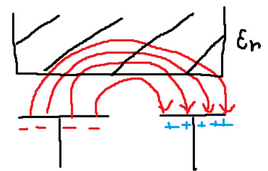
\includegraphics[scale = 0.5]{img/BezkontC.png}
\end{figure}

\subsubsection{Varianty}
\subsubsection*{Nevodivá clonka}
Změna kapacity je malá, mění se jen permitivita
\subsubsection*{Vodivá clonka}
Střední změna kapacity, mezi elektrody jakoby vkládáme další, která není uzemněna, když měníme vzdálenost, chová se to stejně, jak kdybychom zmenšovali vzduchovou mezeru - tj. bude se měnit kapacita(s velkou citlivostí) z důvodu změny vzdálenosti mezi elektrodami.\\
\subsubsection*{Vodivá clonka uzemněná}
Spojená s jednou s elektrod. Velká změna kapacity, výstupní kapacita je nepřímo uměrná vzdálenosti, 2x větší citlivost.\\

\begin{figure}[h!]
    \centering
    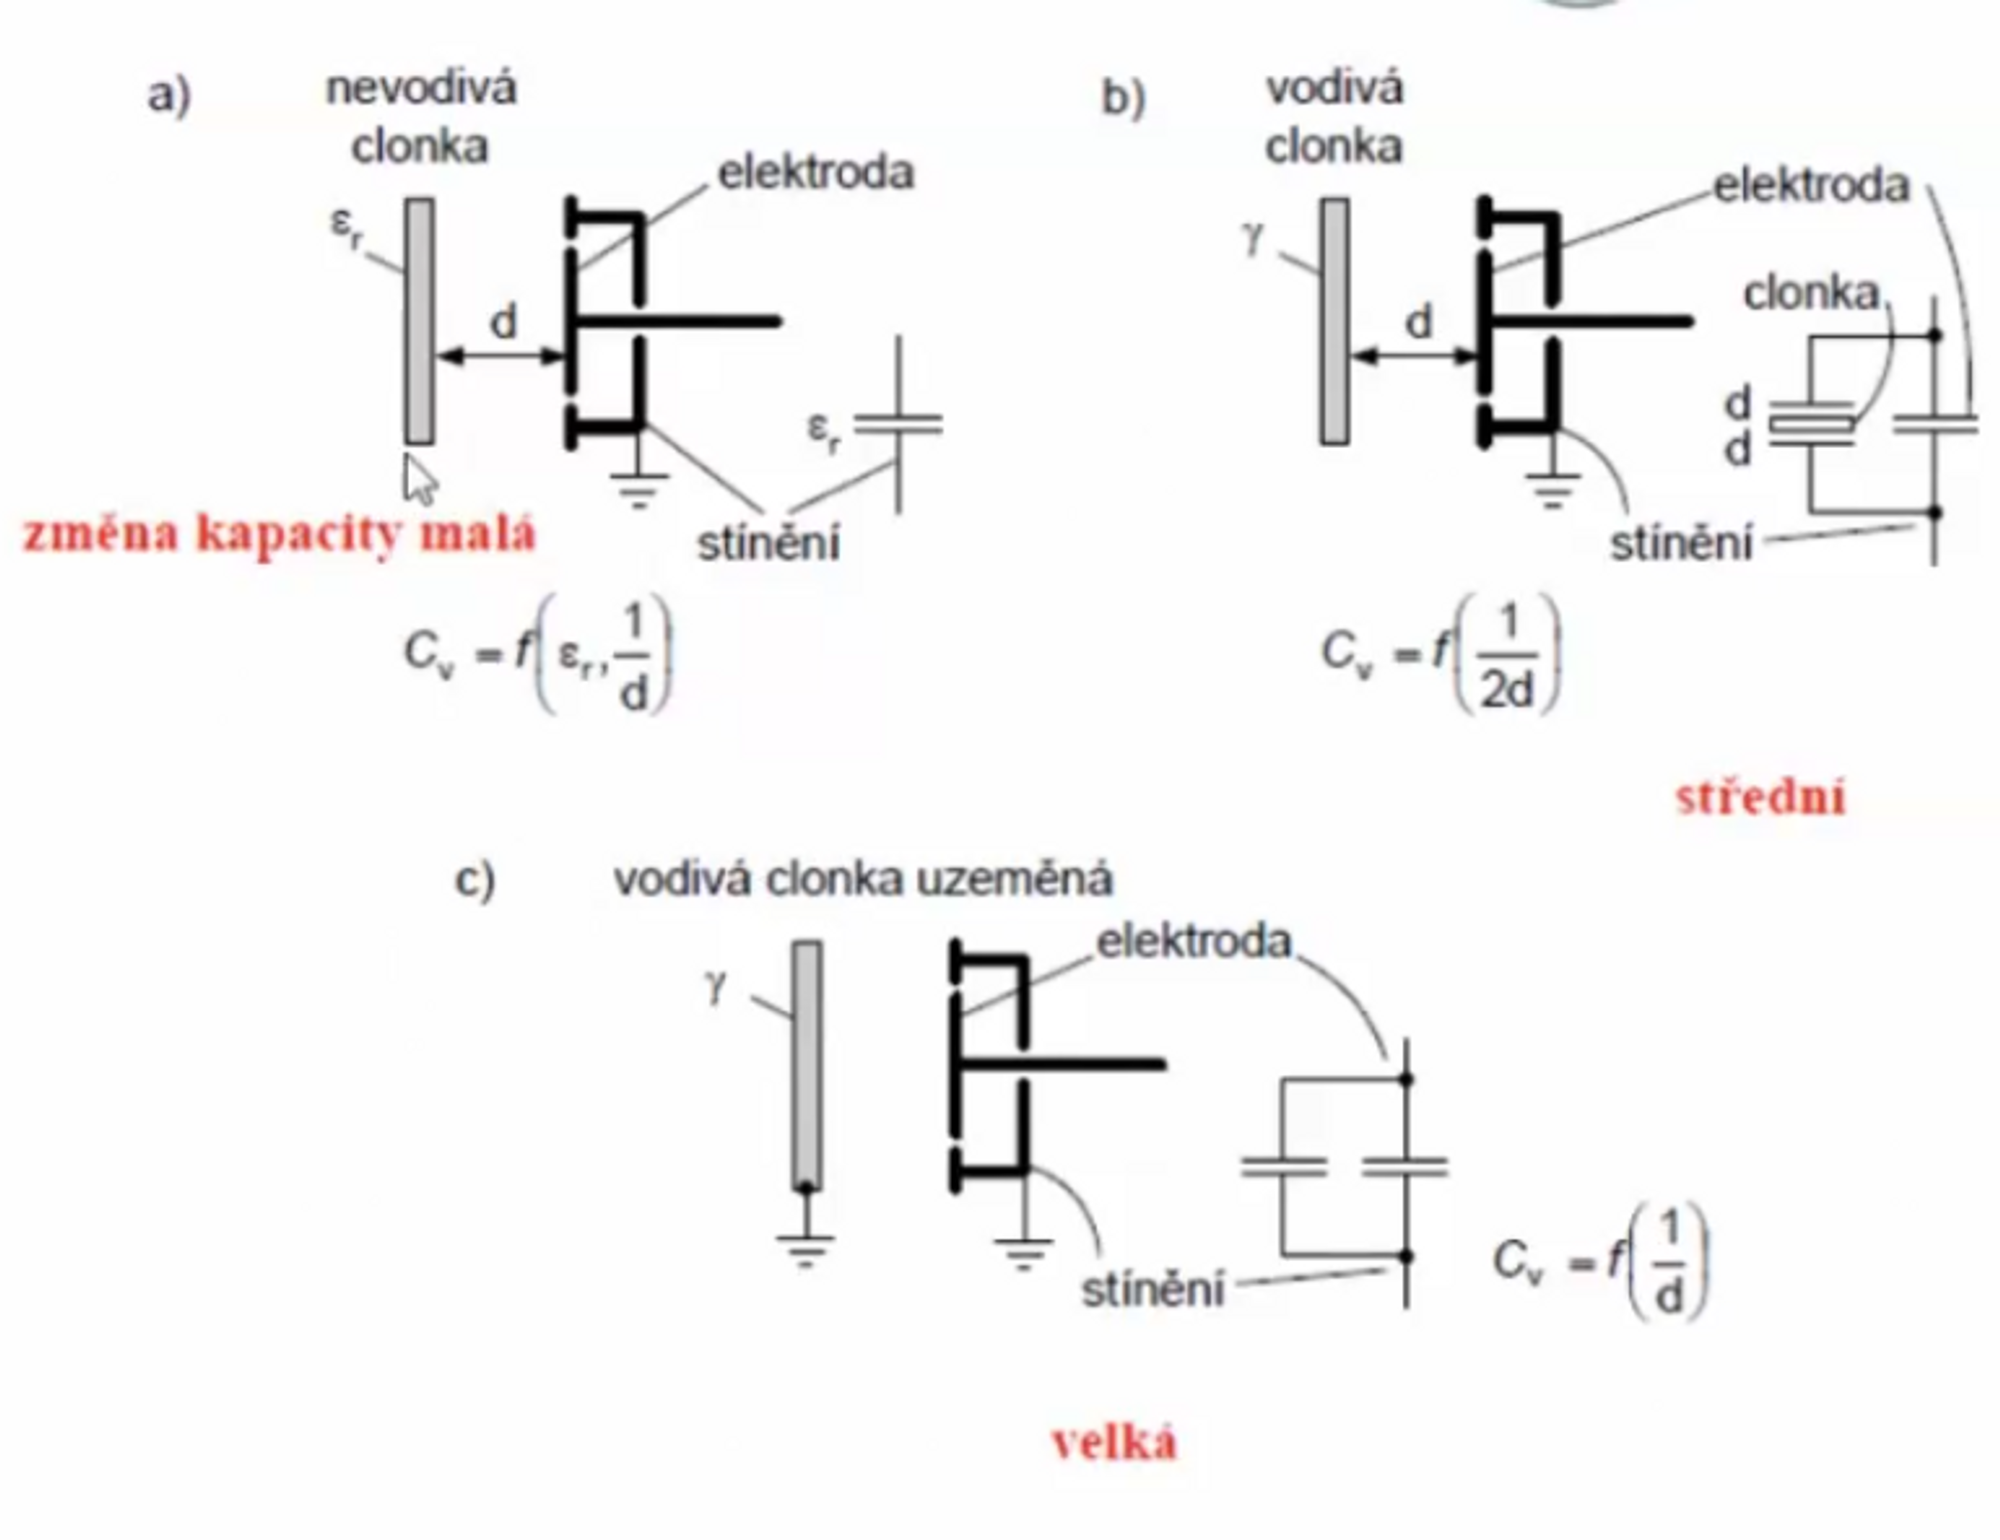
\includegraphics[scale = 0.2]{img/VariantyCpol.png}
\end{figure}
\subsubsection{Použití}
Měření hladiny vody, olejů, sypkých hmot přes stěnu nádrže.\\
Kontrola počtu/přítomnosti výrobků na balících linkách.\\


\section{Měření polohy - principy optické, magnetické, ultrazvukové}


\section{Měření vibrací, rychlosti, zrychlení, akcelerometry, snímače úhlové rychlosti }


\section{Tenzometry, snímače síly, hmotnosti, momentu a tlaku }


\section{Měření průtoku, základní principy objemových, rychlostních a hmotnostních průtokoměrů}


\section{Kontaktní snímače teploty (dilatační, odporové, termoelektrické)}


\section{Měření záření (tepelné a kvantové snímače IR záření, snímače ionizujícího záření)}


\section{Chemické snímače}